\chapter{Implementation Approach}
\label{chap:implementation}
\lhead{\emph{Implementation Approach}}

%The key question to be addressed in this chapter is: "How do I plan to achieve what I have outlined in the previous chapter".

%This chapter should comprise around 5000 words and specify your planned implementation approach. Again all sections below are suggestions and will vary significantly from project to project, the key element to be addressed is the core question of the chapter.

\section{Architecture} \label{sec:Arch}
%Describe the architecture of the solution that you have in mind, including:
%\begin{itemize}
%    \item Technologies involved (e.g., frameworks, programming language). 
%    \item The hardware needed to develop the project (and to support at deployment stage)
%\end{itemize}

%Provide a high level view of the system you have in mind, including any package of classes, what is it responsible for and what other packages it communicates to. Provide a high level view of the database (or structure) needed to support the project, including what each table/document is responsible for and the hierarchy among them. You need to be as specific here as you can, why? Because this will aid you in identifying parts of the project you are vague on, this may be fine for some components but cause problems in term 2 for others. If you have hardware element in your project this is also where you provide a high level view of how these elements integrate into the project. So for a project that is cyber-physical you will have both a hardware and software architectural diagram. N.B. This is NOT a full system design but a high level overview of what you can credibly develop. This architecture should be informed by prototyping activity. 

%Some of the implementation focused projects may describe how do you envision tackling the functional requirements of your project via a set of use-cases. DFDs are also helpful here to understand elements of your project that may cause problems. You should describe the role of the different parts of the architecture of the solution, and the interaction among them.

Designing a software architecture is a crucial step of creating software. This will attempt to illuminate any uncertainties that come up with the functionality or implementation. Planning out the architecture before coding often results in a more stable and scalable software. This section will be dedicated to explaining how the project is going to work. The technologies and languages used for this project will be introduced as needed. High level diagrams and class diagrams will accompany the explanation, these diagrams will most likely change during the implementation phase as it would be rather amazing if I got every thing correct here.

The project will be written in C++ as it is a binary compiled language resulting in fast execution of code, this is required as synchronisation takes up a reasonable amount of execution time. C++ has libraries for dealing with networking and threads therefore building an API will be no problem. I also plan on doing a NodeJs module for easy integration with the API using any NodeJS application, this will be done in JavaScript.

\begin{figure}[!h]
  \centering
      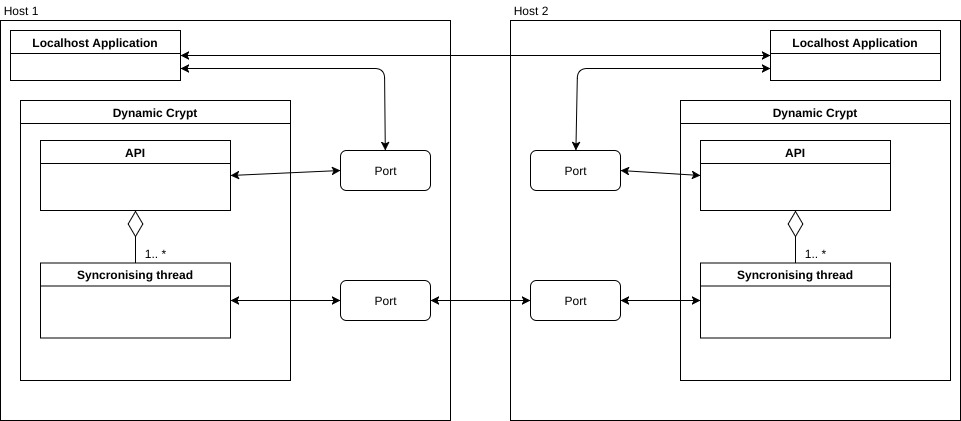
\includegraphics[width=1\textwidth]{Figures/basic-2hosts.jpg}
  \caption[Two hosts using Dynamic Crypt System]{Two hosts using Dynamic Crypt System}
  \label{fig:2hostsbasic}
\end{figure}

\FloatBarrier

The diagram \ref{fig:2hostsbasic} shows a very high level overview of the system in action. There are two hosts in this example. Each host has a localhost Application which is any application that uses the API, it can be a python web application, NodeJS web application, PHP web application etc... 

Each host has a Dynamic Crypt software running which is what this project is about. 

The Dynamic Crypt has two main sort of components if you like. The API which is responsible for communication between applications running on localhost only for security purposes. The localhost applications communicate with the API through a port that will be configured with iptables to only be available for local addressees only so 127.0.0.1 only. 

The Synchronising thread "component" is a single Tree Parity Machine as well as the necessary functionality required for networking and synchronisation between the partner thread of the other host. Each synchronising thread will have its own unique id as well as the partner thread id, IP, port etc.. from the other host in order to be able to send packets directed at the partner thread. This is needed because there will be multiple instances or threads for each host connected to a host. In the host 1 to host 2 example there will most likely be only ten threads synchronising with each other this is to ensure a steady supply of encryption keys, this number of threads for each host may change during the implementation phase. 

How all of this works is going to be similar to the following. 

Host 1: Localhost application establishes a connection with Host 2: Localhost application using standard methods. 

When local Host 1: Localhost application wants to use dynamic encryption to send data to Host 2: Localhost application it contacts the Host 1: Dynamic Crypt API with an init request. 

Host 1: Dynamic Crypt API takes note of Host 1: Localhost application details such as the applications name or port number to distinguish the application from other local host applications as will be demonstrated in a later example. and initialises ten Synchronising threads. The API associates this list of synchronising threads with the application and sends back the details of each thread, the port the threads will use and the IP of Host 1 to Host 1: Localhost application.

Host 1: Localhost application then essentially forwards this information to Host 2: Localhost application which will know that this is an dynamic synchronisation init request and will forward that information to Host 2: Dynamic Crypt API through the Host 2: Dynamic Crypt API port. The Host 2: Dynamic Crypt API will initialise ten Synchronising threads and assigns a partner to them which is essentially the partner id of one of the Host 1: Dynamic Crypt threads.

Host 2: Dynamic Crypt threads will send a request to Host 1: Dynamic Crypt threads. The Thread manager will then forward the info to each thread assigning the partners thread id for Host 1 threads. Now synchronisation between threads will occur how synchronisation occurs is discussed in the research phase but I will provide a diagram shortly.

When a thread is synchronised the API of both hosts will notify the corresponding Localhost application that dynamic synchronisation may occur. The key of the synchronised thread is saved in the API and the thread is forced to desynchronise and begin synchronisation again in order to get a new key. These keys will be added in a queue on both of the hosts API.

The Localhost application can now call the API with an encrypt message request and pass a message to be encrypted. The API uses a key to encrypt a message then the key is discarded from the API, the encrypted message is returned to the Localhost application for ready for sending. 

The message arrives at the other Localhost application. The Localhost application will send a decrypt request to the API with the encrypted message. The API will use the appropriate key to decrypt the message and send it back to the Localhost application. 









\begin{figure}[!h]
  \centering
      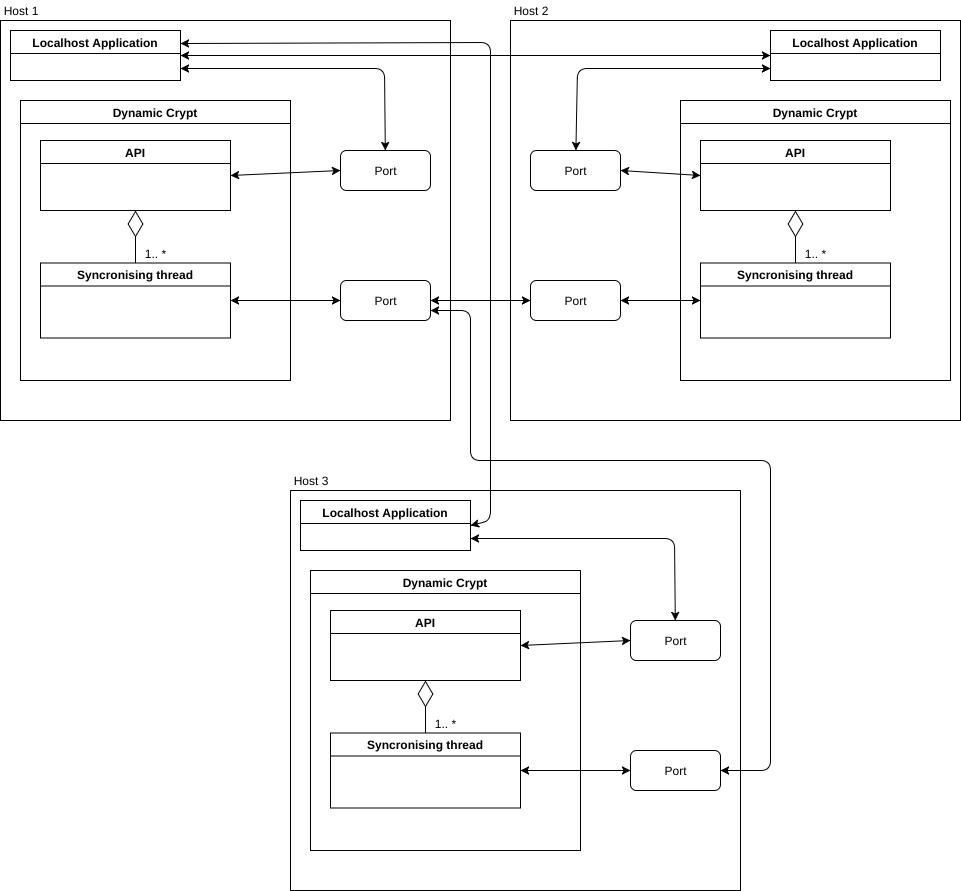
\includegraphics[width=1\textwidth]{Figures/basic-3hosts.jpg}
  \caption[Host one using Dynamic Crypt System with host two and three at the same time]{Host one using Dynamic Crypt System with host two and three at the same time}
  \label{fig:3hostsbasic}
\end{figure}

\FloatBarrier

The diagram \ref{fig:3hostsbasic} demonstrates how dynamic encryption can be implemented when Host 1: Localhost application wishes to send dynamically encrypted information between Host 2 and Host 3 simultaneously. Because Host 1 is attempting to use dynamic encryption to communicate between Host 2 and Host 3 only this means that Host 2 and Host 3 are not aware of each other as there is no need for them to communicate.

This works in quite a similar fashion as with only two hosts but now there are three.

Host 1: Localhost application establishes a connection with Host 2: Localhost application and Host 1: Localhost application establishes a connection with Host 3: Localhost application using standard methods more than likely this will happen one after the other as extra data might be required from Host 3, however there is not going to cause any problems doing it at the same time. 

Host 1: Localhost contacts the Host 1: Dynamic Crypt API with an init request twice one for Host 2 and Host 3. In the init request Host 1: Localhost application also provides any name for Host 2 and Host 3 to distinguish quickly between the two later on.

Host 1: Dynamic Crypt API takes note of Host 1: Localhost application details such as the applications name or port number and the name given to Host 2 and Host 3, and initialises ten Synchronising threads for Host 2 and another ten Synchronising threads for host 3. The API associates this list of synchronising threads with the application and sends back the details of each thread, the port the threads will use, the IP of Host 1 and lastly the name given to Host 2 and Host 3 to Host 1: Localhost application. These details are sent back for Host 2 and Host 3 separately to allow for easy growth since Host 1 might want to dynamically encrypt information and send it to Host 3 much later than Host 2.

Host 1: Localhost application then essentially forwards this information to Host 2: Localhost application and Host 3: Localhost application these will know that this is an dynamic synchronisation init request and will forward that information to Host 2: Dynamic Crypt API through the Host 2: Dynamic Crypt API port and Host 3: Dynamic Crypt API through the Host 3: Dynamic Crypt API port. The Host 2: Dynamic Crypt API and Host 3: Dynamic Crypt API will each initialise ten Synchronising threads and assign a partner to them which is essentially the partner id of one of the Host 1: Dynamic Crypt threads.

Host 2: Dynamic Crypt threads will send a request to Host 1: Dynamic Crypt threads followed by another request from Host 3: Dynamic Crypt threads to Host 1: Dynamic Crypt threads. The Thread manager will then forward the info to each thread assigning the partners thread id for Host 1 threads. Now synchronisation between threads will occur.

The last three steps are identical as in the last example.



\begin{figure}[!h]
  \centering
      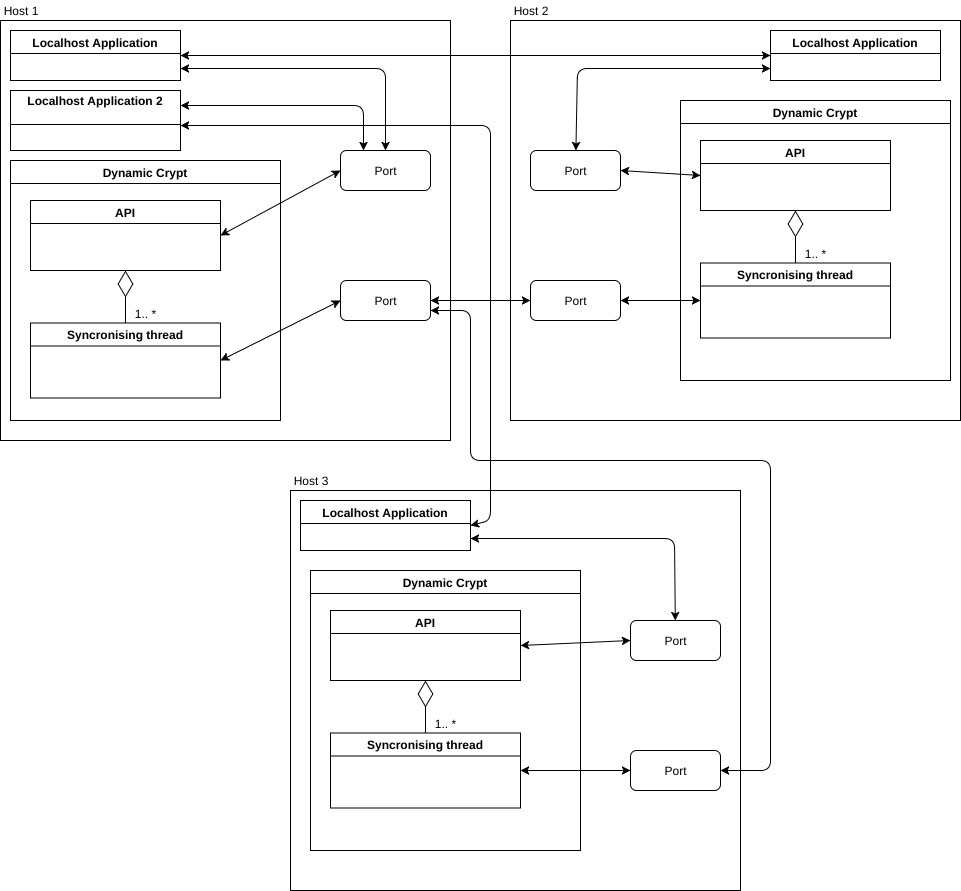
\includegraphics[width=1\textwidth]{Figures/basic-3hosts-2apps.jpg}
  \caption[Host one using Dynamic Crypt System with host two and three with different applications using the API]{Host one using Dynamic Crypt System with host two and three with different applications using the API}
  \label{fig:3hostsbasic2apps}
\end{figure}

\FloatBarrier

The diagram \ref{fig:3hostsbasic2apps} is quite similar to the last example where as in this case there are two local host applications running on Host 1: In this case localhost application 1 is using the dynamic encryption system to send data to Host 2 and localhost application 2 is using the dynamic encryption system to send data to Host 3. They both use the same API and therefore this example is quite similar to the previous one.

Host 1: Localhost application 1 establishes a connection with Host 2: Localhost application using standard methods.
Similarly Host 1: Localhost application 2 establishes a connection with Host 3: Localhost application using standard methods.

Host 1: Localhost application 1 contacts the Host 1: Dynamic Crypt API with an init request. 
Host 1: Localhost application 2 contacts the Host 1: Dynamic Crypt API with an init request. 

Host 1: Dynamic Crypt API takes note of Host 1: Localhost application 1 details such as the applications name or something to distinguish it from Host 1: Localhost application 2, and initialises ten Synchronising threads. The API associates this list of synchronising threads with the application and sends back the details of each thread, the port the threads will use and the IP of Host 1 to Host 1: Localhost application 1 and similar but different values are sent to Host 1: Localhost application 2 as well. 

Host 1: Localhost application 1 forwards this information to Host 2: Localhost application which will know that this is an dynamic synchronisation init request and will forward that information to Host 2: Dynamic Crypt API through the Host 2: Dynamic Crypt API port. 
Host 1: Localhost application 2 forwards this information to Host 3: Localhost application which will know that this is an dynamic synchronisation init request and will forward that information to Host 3: Dynamic Crypt API through the Host 2: Dynamic Crypt API port. 
The Host 2: Dynamic Crypt API and The Host 3: Dynamic Crypt API will initialise ten Synchronising threads and assigns a partner to them which is essentially the partner id of one of the Host 1: Dynamic Crypt threads.

Host 2: Dynamic Crypt threads will send a request to Host 1: Dynamic Crypt threads followed by another request from Host 3: Dynamic Crypt threads to Host 1: Dynamic Crypt threads. The Thread manager will then forward the info to each thread assigning the partners thread id for Host 1 threads. Now synchronisation between threads will occur.

The last three steps are identical as in the first example.



From the three use case examples the API must be able to support:
\begin{itemize}
    \item A single localhost application connecting with another dynamic encryption system.
    \item A single localhost application connecting with multiple other dynamic encryption systems.
    \item Multiple localhost applications connecting with other dynamic encryption systems.
    \item Multiple localhost applications connecting with multiple other dynamic encryption systems per each local host application.
\end{itemize}

\begin{figure}[!h]
  \centering
      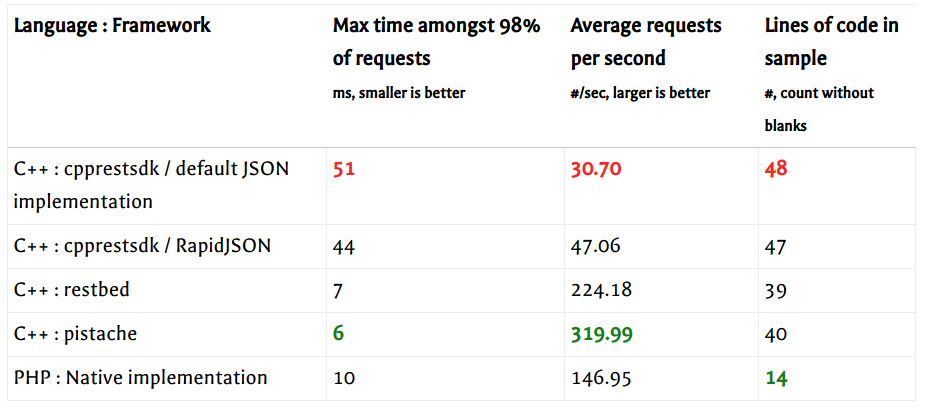
\includegraphics[width=1\textwidth]{Figures/cppframeworks.png}
  \caption[Comparison of different C++ rest frameworks]{Comparison of different C++ rest frameworks\cite{Crestframeworks}}
  \label{fig:Crestframeworks}
\end{figure}

\FloatBarrier

In order to build a proper API I will use a framework as making one from scratch would be too time consuming. There are not many C++ only rest APIs frameworks so the choice was not too difficult. 
Table \ref{fig:Crestframeworks} shows the most popular C++ rest frameworks. Cpprestsdk is made by Microsoft and is generally the most popular one to use. However I have tried installing the library and had issues compiling the examples provided on their GitHub a simple hello world server worked perfectly but the rest API example had issues. This is perhaps for the better that I was unable to get it to work and had to find other frameworks to work with. I stumbled upon the websites that the table is from and the framework Pistache \cite{pistache} seems to be leaps ahead of Cpprestsdk having a low request time of only 6 milliseconds and a large 320 requests per second capability which is what I need for this project and considering that it will take quite a lot of requests to synchronise tree parity machines. Fortunately I was able to install the library correctly and the example rest API code for Pistache compiled and worked correctly.

Therefore I will be using Pistache as the rest API part of this project and the tree parity part of the code also since I wanted my software to utilise two ports.



\begin{figure}[!h]
  \centering
      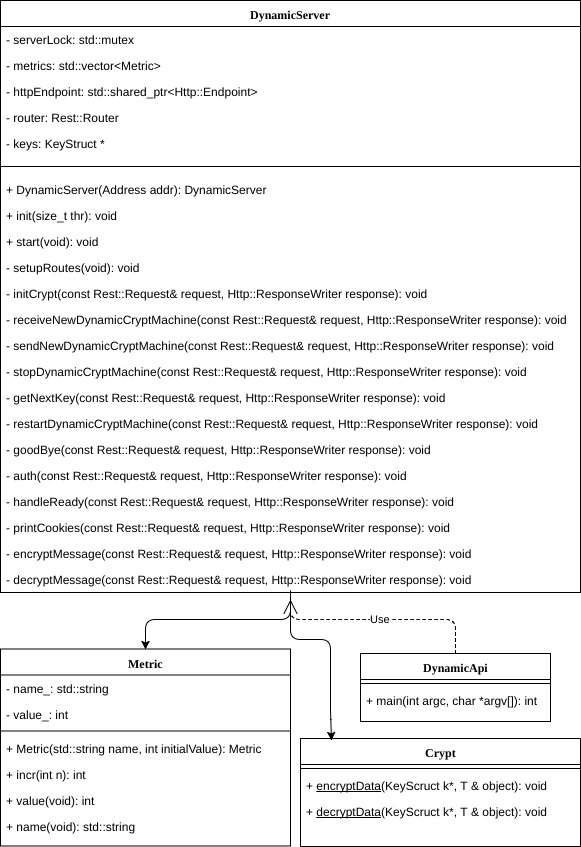
\includegraphics[width=1\textwidth]{Figures/API.jpg}
  \caption[Rest API class diagram]{Rest API class diagram}
  \label{fig:myapi}
\end{figure}

\FloatBarrier

The class diagram \ref{fig:Crestframeworks} demonstrates roughly how the API will look like. The variables at the top of the DynamicServer class are mostly used for the library. serverLock is to prevent issues with threads changing the same variable at the same time. metrics is for measuring various server performances this uses the Metric class defined in the diagram. httpEndpoint is a pointer used by the framework internally. router is used for handling different routes in the setupRoutes function. keys is a struct array that has the generated encryption key from the tree parity machine, the id of the tree parity machine and a status whether it was sent of or not more properties will most likely be added in the implementation phase to this struct.

The functions after setupRoutes are all route handlers that will need to be associated with a route in the setupRoutes function. initCrypt function will tell the tree parity machine handler to setup the tree parity machines. receiveNewDynamicCryptMachine is when a different host setup the tree parity machines and sends you ids and other information to allow for partnering of this hosts tree parity machines. sendNewDynamicCryptMachine is the opposite of the previous this time the api is sending info of its tree parity machines to another host. stopDynamicCryptMachine this is used when the application believes it doesnt need any more new keys for dynamic encryption so the synchronisation will cease to avoid expensive unnecessary operations. getNextKey will send the next if available key to the application. restartDynamicCryptMachine would be typically called after stopDynamicCryptMachine to generate more keys once again. goodBye will be called when the application doesn't need to use the API anymore this will remove any references and any tree parity machines relating to the application. When the application disconnects from the API a similiar set of instructions will also occur. auth is when authorisation will be implemented for increased security. handleReady is more of a test function to determine if server is up and running. printCookies will most likely never be used. 

The Metric class is used for saving different server metrics. A metric has a name, value and increment amount.

Lastly the DynamicApi class holds the main method that initialises the server.





\begin{figure}[!h]
  \centering
      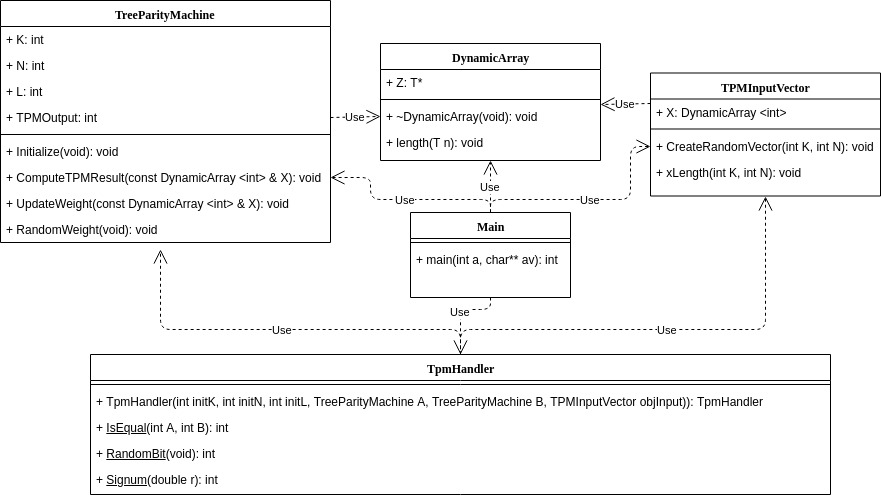
\includegraphics[width=1\textwidth]{Figures/TreeParityMachine.jpg}
  \caption[Tree Parity Machine synchronisation class diagram]{Tree Parity Machine synchronisation class diagram}
  \label{fig:tpmClassDiagram}
\end{figure}

\FloatBarrier

this is reference to diagram\ref{fig:tpmClassDiagram}.







\section{Risk Assessment}
%Identify any potential risk precluding you from successfully complete your project. This section is really important and often neglected by students resulting in fatal risks occurring in some projects. Make sure to give this section the time it requires. Classify the risk according to their importance, possibility of arising and enumerate the decisions you can make to anticipate them or mitigate them (in case they finally arise). Table \ref{tab:ProjRisks} may help with this classification. This section should include your mitigation approach for any critical risks.

%\begin{table}[h]
%\centering
%\scriptsize
%\caption{Initial risk matrix}
%\begin{tabular}{|p{2cm}|p{2cm}|p{2cm}| p{2cm} |p{2cm}| p{2cm}|}
%\hline \bf Frequency/ Consequence & \bf 1-Rare & \bf 2-Remote & \bf 3-Occasional & \bf 4-Probable & \bf 5-Frequent\\ [10pt]

%\hline \bf 4-Fatal & \cellcolor{yellow!50} & \cellcolor{red!50} & \cellcolor{red!50} & \cellcolor{red!50} &\cellcolor{red!50} \\ [10pt]

%\hline \bf 3-Critical &\cellcolor{green!50} & \cellcolor{yellow!50} & \cellcolor{yellow!50} & \cellcolor{red!50} &\cellcolor{red!50} \\ [10pt]

%\hline \bf 2-Major & \cellcolor{green!50} & \cellcolor{green!50} & \cellcolor{yellow!50} &\cellcolor{yellow!50} &\cellcolor{red!50} \\ [10pt]

%\hline \bf 1-Minor & \cellcolor{green!50} & \cellcolor{green!50} & \cellcolor{green!50} &\cellcolor{yellow!50} &\cellcolor{yellow!50} \\ [10pt]
%\hline
%\end{tabular} \\
%\label{tab:ProjRisks}
%\end{table}

\section{Methodology}
%Describe your personal approach on how to tackle the different parts of this project, including:
%\begin{itemize}
%    \item How to tackle the needed research to fulfill the background chapter. 
%    \item How to set up your Computer Science skills to the project needs (e.g., describe your plan to learn any new technology involved on the project that you are not familiar with). 
%    \item What core project managing approach will you follow (e.g., Waterfall, Scrum, etc).
%\end{itemize}

\section{Implementation Plan Schedule}
%Come up with a schedule for the remaining time (including second semester), so as to describe how do you envision to achieve the implementation of your project by the end of semester 2. This plan SHOULD be ambitious but MUST be realistic and SHOULD be informed by early prototyping and MUST be discussed with your term 1 supervisor.

\section{Evaluation}
%Come up with an evaluation plan that allows you to measure how much have you actually achieved the goals of your project. This again is a section that is often neglected where students loose marks. How do you plan to measure the output of your project? A binary it works/does not work is insufficient. You need to be able to quantify the success against both the functional requirements and the initial idea. These are not the same as you may meet all function requirements outlined but not solve the overall problem because you have failed to revisit these and update them with new information which you learn as you are developing the project.

\section{Prototype}
%Although you do not have a fully functional project yet, you should show wireframes, snapshots or representation on how do you envision your project to look once the implementation phase has been completed. The nature of this section will vary significantly from project to project and can include anything from code snippets to snapshots of service deployments. Any prototyping you have done during the term should be summarized here that has not been captured in earlier sections. For example if you are planning to host your project using AWS in an EC2 instance you should have at least created a "hello world" setup to determine the basics, this probably should have been discussed in section \ref{sec:Arch}.